%todo: compare to the plan from the meeting:
%25+5min

%explain in the presentation:

%{Algorithm! abstract aufzeichnen
%abstracter code (algo_sketch) zusammen mit spezifikation und "l"
%mit phases
%refinement von phase 1
%und bei 2+3 pläne} 5min
%Bibliotheken vorstellen, Wahl begründen
%--> Graphformalisierungen: directed vs. undirected edges in both phases. Welche gibt es alle?
%edge labels, i.e. a third field besides start node and end node 5min
%MST lemma zeigen, wieso nicht Graph_Theory? 5min
%was ist der projektstatus? 5min
%maybe a slide about the commit count?
%add dfs-sublocale statement to plans. "This is already proven. However, the set membership must be implemented..."

\documentclass[%handout,
	sans,
	12pt,
	%slidescentered,% center text on slide
	%draft,			% compile as draft version
	%notes,			% include nodes in slides
	%compress		% compress navigation bar
]{beamer}

\beamertemplatenavigationsymbolsempty

\usetheme{default}
\usecolortheme{orchid}
\setbeamertemplate{frametitle}
{
    \vspace*{1.5em}\insertframetitle\vspace*{-1.5em}
}
\setbeamertemplate{footline}[frame number]

\usepackage[T1]{fontenc}
\usepackage[utf8x]{inputenc}

\usepackage{mathpazo}
\usepackage[british]{babel}
\usepackage{csquotes}

\newcommand{\high}[1]{{\usebeamercolor[fg]{structure} #1}}
\newcommand{\bad}[1]{\textcolor{red}{#1}}
\newcommand{\gray}[1]{\textcolor{darkgray}{#1}}
\newcommand{\black}[1]{\textcolor{black}{#1}}

\usepackage{amsmath,amssymb}
\usepackage{upgreek}
\usepackage{booktabs}
\usepackage{hyperref}
\usepackage{graphicx}
\usepackage{colortbl}
\usepackage{url}
\usepackage{setspace}
\usepackage{wrapfig}
\usepackage{tabularx}
\usepackage{xspace}
\usepackage{mathpartir}

\usepackage{tikz}
\usetikzlibrary{trees, positioning}
\usetikzlibrary{shapes.geometric}

\usepackage{isabelle,isabellesym}
\isabellestyle{it}
\def\isacartoucheopen{}%
\def\isacartoucheclose{}%

\newcommand{\NN}{\mathbb{N}}
\newcommand{\QQ}{\mathbb{Q}}
\newcommand{\RR}{\mathbb{R}}
\newcommand{\CC}{\mathbb{C}}
\renewcommand{\epsilon}{\varepsilon}
\renewcommand{\phi}{\varphi}
\def\braces#1{[#1]}
\newcommand{\wrt}{w.\,r.\,t.\xspace}
\newcommand{\eg}{e.\,g.\xspace}
\newcommand{\ie}{i.\,e.\xspace}
\DeclareMathOperator\caret{\char`\^}

\newcommand{\hastype}{\,:\,}
\newcommand{\cons}{::}
\newcommand{\corrto}{\overset{\scriptscriptstyle\wedge}{=}}
\newcommand{\listapp}{\mathbin{@}}
\newcommand{\listnil}{[\hskip0.3mm]}
\newcommand{\listnth}{\mathbin{!}}
\newcommand{\expectation}{\text{\upshape E}}

\usepackage{manfnt}
\newenvironment{danger}{\medbreak\noindent\hangindent=2pc\hangafter=-2%
  \clubpenalty=10000%
  \hbox to0pt{\hskip-\hangindent\hskip0.25em\raisebox{-0.25em}[0pt][0pt]{\dbend}\hfill}\small\ignorespaces}%
  {\medbreak\par}
  %\raisebox{-1.05em}[0pt][0pt]{\Huge\hskip.15em \stixdanger}

\newcommand{\etAl}{\textit{et al.}\xspace}

%\definecolor{mybg}{rgb}{0.9,0.9,0.9}
\definecolor{mybg}{rgb}{1,1,1}
\setbeamercolor{background canvas}{bg=mybg}

\title{Verification of an Approximation Algorithm for the Metric Travelling Salesperson Problem}
\author{\normalsize Fabian Hellauer}
\institute[]{\footnotesize Technische Universität München}
\date{\footnotesize16 October 2019}

\begin{document}

\maketitle

\begin{frame}
\begin{center}
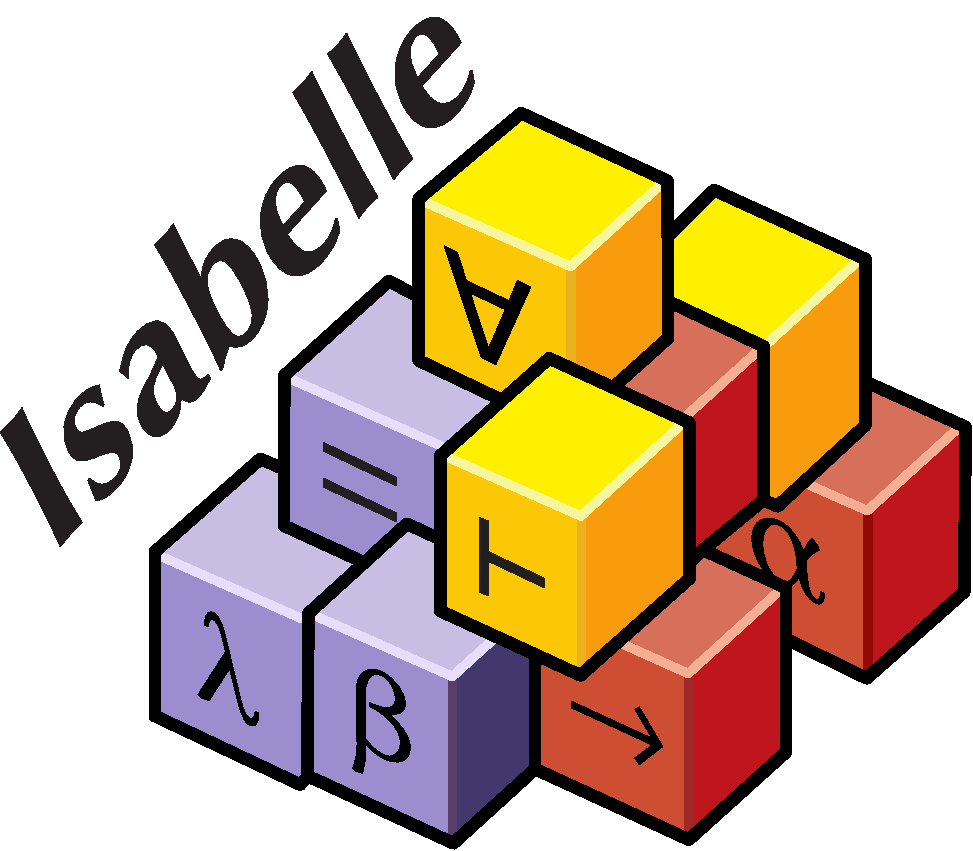
\includegraphics[width=5cm]{isabelle.pdf}
\end{center}
\end{frame}

\tableofcontents	%to-do: remove

\newcommand{\pivot}[1]{{\color{red}#1}}
\newcommand{\ltpiv}[1]{{\color{blue}#1}}
\newcommand{\gtpiv}[1]{{\color{olive}#1}}

\section{Isabelle}
\section{Metric TSP}
\section{Approximation Algorithms}
\section{MST Heuristic} %advance the 2-approx-proof during the phases or maybe add another slide?
    \subsection{MST Generation}
    \subsection{Tour Search}
    \subsection{Duplicate Removal}
    \subsection{Resource Usage Analysis?}%or maybe at the very end?
\section{Results}
    \subsection{Algorithm Sketch} %"to see how the specification and algorithm look in the framework"
    %to-do: how to handle context here?
    \subsection{Library Connections}
    \subsection{Simplification of Phase Two?}% not really my work, but something which slowed me down...
\section{Plans}
    \subsection{Input Generation} %how to generate input that fulfils the specification
    %maybe also mention the drilling robot during this slide
    \subsection{Last Pieces of a DFS Invariant}
    
% add draft slide from the meeting

\section{---------slides from here---------}
\section{Verification of Algorithms}
\begin{frame}{Verification of Algorithms}
Reasons:
\begin{itemize}
	\item a basis for reliable software\pause
	\item find mistakes in algorithm explanations\pause
	\item prove that verification of executable programs
	is feasible\ % when using a modern tool like
	 when using 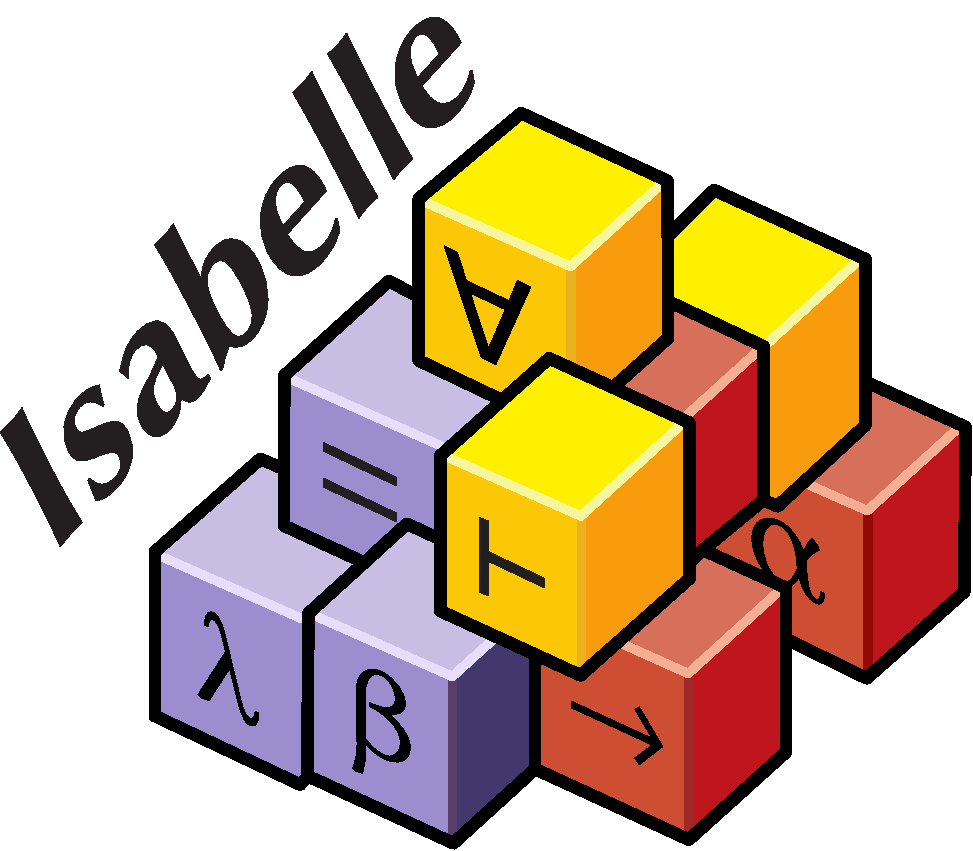
\includegraphics[height=1em]{isabelle.pdf}Isabelle\pause
\end{itemize}
Mathematical results might be a requirement.
%In this case here, from graph theory.
\end{frame}

\section{Metric TSP}
\begin{frame}
	TSP is the problem of finding a tour of minimal cost within a graph.\\\pause
	We consider the special case where the nodes form a \textit{metric} with their weights.\\\pause
	In particular,\pause
	\begin{itemize}
		\item \textit{weight} is total
		% All TSP cities are connected by an edge, in other words we require the graph to be complete.
		\item $\textit{weight}\ v_1\ v_3\ \leq\ \textit{weight}\ v_1\ v_2\ +\ \textit{weight}\ v_2\ v_3$
		\item $0\ \leq\ \textit{weight}\ v_1\ v_2$\pause
	\end{itemize}
	In such a graph, the cost of a \textit{minimum spanning tree} is a lower bound on the optimal tour cost.
\end{frame}

\section{Approximation Algorithms}
\begin{frame}{Approximation Algorithms}
	What are Approximation Algorithms?\pause%to-do: explain based on (metric) TSP
	\vspace{1em}
	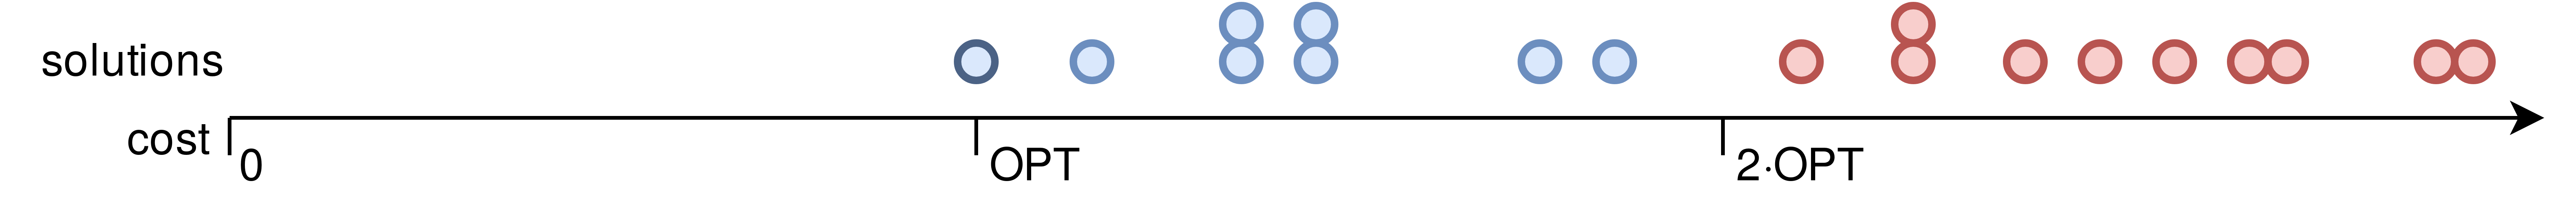
\includegraphics[width=\linewidth]{OPT_line}
	%OPT is the performance of an *actual* algorithm, namely the brute-force algorithm that tries all exponentially many node sequences.
	\vspace{1em}\pause %Since we consider undirected graphs, the reverse of a TSP tour is also a TSP tour (I omitted these duplicates in the graphic)
	
	\high{Good solutions for NP-complete problems in polynomial time!}
\end{frame}

\section{Algorithm Explanation}
\begin{frame}
\begin{center}
	\huge\high{Algorithm Explanation}
\end{center}
\end{frame}

\subsection{MST Generation}
\begin{frame}{MST Generation}\pause
Consider a complete undirected graph and its minimum spanning tree $T$.\pause%or rather one of its minimum spanning trees


to-do: graphic
\begin{isabelle}
\isacommand{lemma}\isamarkupfalse%
\ minimum{\isacharunderscore}spanning{\isacharunderscore}tree{\isacharunderscore}le{\isacharunderscore}OPTWEIGHT{\isacharcolon}\isanewline
\ \ \isakeyword{assumes}\ {\isacartoucheopen}minimum{\isacharunderscore}spanning{\isacharunderscore}tree\ {\isacharparenleft}ind\ F{\isacharparenright}\ {\isacharparenleft}ind\ {\isacharparenleft}symhull\ E{\isacharparenright}{\isacharparenright}{\isacartoucheclose}\isanewline
\ \ \isakeyword{assumes}\ {\isacartoucheopen}{\isadigit{2}}\ {\isasymle}\ card\ V{\isacartoucheclose}\isanewline
\ \ \isakeyword{shows}\ {\isacartoucheopen}set{\isacharunderscore}cost\ F\ {\isasymle}\ OPTWEIGHT{\isacartoucheclose}
\end{isabelle}
\end{frame}

\subsection{Tour Search}
\begin{frame}{Tour Search}
Find an edge sequence which\pause
\begin{itemize}
	\item uses exactly the MST's edges, each of which twice\pause
	\item visits every node\pause
	\item starts and ends at the same node\pause
\end{itemize}
This sequence is then called a \textit{pretour}.\pause

Its cost is twice the cost of the MST's edges.
%And the MST's edges are, as mentioned, less than the cost of an optimal tour.
\end{frame}

\subsection{Duplicate Removal}
\begin{frame}{Duplicate Removal}
Transform the pretour into a TSP tour:
%typically we require TSP tours to visits each node exactly once. Our sequence doesn't do that yet.
\begin{itemize}
	\item remove duplicate visits, replace them by shortcuts.
	%That means that when the sequence goes to an already visited node, we instead jump to the next one
\end{itemize}
These shortcuts always exist and do not increase the cost. %That is why we require a complete metric graph
\end{frame}

\subsection{Resource Usage}
\begin{frame}{Resource Usage}
\begin{itemize}
	\item MST generation: $\mathcal{O}(|E| \log |E|) = \mathcal{O}(n^2 \log (n^2)) = \mathcal{O}(2(n^2 \log n)) = \mathcal{O}(n^2 \log n)$%We use Kruskal's, which sorts edges by comparisons
	\item Tour: $\mathcal{O}(n)$ %This is the number of edges in the MST. We discuss later how we can arrange the edges in time linear to this, to-do: Is this actually covered?
\end{itemize}
overall: $\mathcal{O}(n^2 \log n)$
\end{frame}

\section{Results}
%What I did in the setting of this algorithm
\begin{frame}
\begin{center}
	\huge\high{Results}
\end{center}
\end{frame}

\subsection{Algorithm Sketch}
\begin{frame}{Algorithm Sketch}%to-do: rename to "Specification"?
%We have a fixed graph here, OPT depends on it
\begin{isabelle}
	\isacommand{definition}\isamarkupfalse%
	\ two{\isacharunderscore}approx\ \isakeyword{where}\isanewline
	\ \ {\isacartoucheopen}two{\isacharunderscore}approx\ {\isacharequal}\ SPEC\ {\isacharparenleft}{\isasymlambda}T{\isachardot}\ is{\isacharunderscore}tour\ T\ {\isasymand}\ cost\ T\ {\isasymle}\ OPT\ {\isacharplus}\ OPT{\isacharparenright}{\isacartoucheclose}%explain lack of multiplication
	\vspace{1mm}\pause
	\isacommand{definition}\isamarkupfalse%
	\ algorithm{\isacharunderscore}sketch\ \isakeyword{where}\ {\isacartoucheopen}algorithm{\isacharunderscore}sketch\ {\isacharequal}\isanewline
	do\ {\isacharbraceleft}\isanewline
	\ \ MST\ {\isasymleftarrow}\ SPEC\ {\isacharparenleft}{\isasymlambda}E{\isacharprime}{\isachardot}\ minimum{\isacharunderscore}spanning{\isacharunderscore}tree\ {\isacharparenleft}ind\ E{\isacharprime}{\isacharparenright}\ G{\isacharparenright}{\isacharsemicolon}\isanewline
	\ \ pretour\ {\isasymleftarrow}\ SPEC\ {\isacharparenleft}{\isasymlambda}pT{\isachardot}\ int{\isacharunderscore}vertices\ pT\ {\isacharequal}\ nodes\ G\\ \ \ \ \ {\isasymand}\ cost\ pT\ {\isasymle}\ set{\isacharunderscore}cost\ MST\ {\isacharplus}\ set{\isacharunderscore}cost\ MST{\isacharparenright}{\isacharsemicolon}\isanewline
	\ \ tour\ {\isasymleftarrow}\ SPEC\ {\isacharparenleft}{\isasymlambda}T{\isachardot}\ is{\isacharunderscore}tour\ T\ {\isasymand}\ cost\ T\ {\isasymle}\ cost\ pretour{\isacharparenright}{\isacharsemicolon}\isanewline
	\ \ RETURN\ tour\isanewline
	{\isacharbraceright}{\isacartoucheclose}
\end{isabelle}\pause
\vspace{-4mm}
\begin{theorem}
	\hspace{2.6cm}$\textit{algorithm{\isacharunderscore}sketch} \le \textit{two{\isacharunderscore}approx}$\\
\upshape if $G$ is a complete finite metric graph.
\end{theorem}
\end{frame}

\subsection{Libraries}
\begin{frame}{Libraries}
\begin{enumerate}
	\item \textit{Kruskal}: edges with weight field, undirected/directed
	%to-do: vielleicht unterringeln?
	% I improved this library: I had to reorganise this one to get what I want without unnecessary assumptions.
	\item \textit{DFS\_Framework}: edges are node relations, directed
	\item \textit{Koenigsberg\_Friendship}: edges have a label, undirected
	%We have the worst case in terms of compatibility
	%Worse, there are different notions of "undirected"
	%Koenigsberg-Friendship also forbids loops, for technical reasons
	%It also reinterprets..., Kruskal also has a definition "is_path_undir".
	%to-do: add Noschinski, a third notion of "undirected".
\end{enumerate}
\end{frame}

\subsection{Questions}
\begin{frame}
\begin{center}
	\huge\high{Questions}
\end{center}
\end{frame}

%to-do:
%Problems?
%Conclusion?
%References?

\iffalse
\section{------old from here------}
\section{Results} % what I contributed

\subsection{Vector Spaces}
\begin{frame}{Vector Spaces}\pause
$U \subseteq V$ is a \emph{subspace} iff it is a vector space with $V$'s operations.
%over the same field
\begin{theorem}
\upshape
Let $U \subseteq V$ be a subspace. Then:
\begin{itemize}
	\item $dim_K(U) \le dim_K(V)$.
	\item If $dim_K(U)=dim_K(V) < \infty$, then $U = V$.
\end{itemize} %needed basis extension theorem. As you see, many lemmas I needed were missing.
\end{theorem}\pause
\begin{theorem}
\upshape
Let $n := dim_K(V) < \infty$. Then $V \cong K^n$.
% Note that the map is not explicitely given.
\end{theorem}
\end{frame}

\subsection{Classification of simple algebraic extensions}
\subsubsection{Minimal Polynomial}
\begin{frame}{Minimal Polynomial}%We are in a context where we have fixed L/K and some α∈L
\textbf{definition} \textit{irr} \textbf{where}\\
\hskip1em\textit{irr = (ARG-MIN degree p.}\\
\hskip2em\textit{p ∈ carrier P ∧ monic p ∧ Eval p = $\textbf{0}_L$)}\pause%isabelle does not help in determining "L"
\\[4mm]
\textbf{context}\\
\hskip1em\textbf{assumes} \textit{algebraic}\\%explain algebraic
\textbf{begin}\\[2mm]\pause

(...38 lines later)\\[2mm]
\textbf{lemma} \textit{irr ∈ carrier P} \textbf{and} \textit{monic irr} \textbf{and} \textit{Eval irr = $\textbf{0}_L$}\\\pause
\textbf{and} \textit{irr ≠ \textbf{0}}\\\pause
\textbf{and} \textit{degree irr > 0}\pause
\\[3mm]
Uniqueness of the minimal polynomial takes another 180 lines. %But this is part of an actual proof, so this to be expected
%We keep that "algebraic" assumption for a bit...
\end{frame}

\begin{frame}{Minimal Polynomial II}
Next up:\\\pause
\textbf{lemma} \textit{ring-irreducible irr}\\\pause
\high{The library helps with the proof:}\hskip1em\pause :-)\\\pause%happened rarely
\hskip1em\textit{Eval} is a homomorphism $P → L$.\\\pause
\hskip1em$(irr)$ is the preimage of $\{\textbf{0}\}$ under $Eval$.\\\pause %The set of elements which Eval maps to zero
%Do I need to explain (irr)?
%other library facts tell us that (0) is a primeideal and ↓
\hskip1em Thus, $(irr)$ is a prime ideal.\\[4mm]\pause % The claim follows
(...)\\[4mm]\pause%Some other transformations
\begin{theorem}
	$P/(irr) \cong K(\alpha)$%If \alpha is algebraic
\end{theorem}%overall close to 400 lines because I had to define algebraic first
%There is actually quite a bit about such quotient structures
\end{frame}

\section{Problems}
\begin{frame}{Problems}\pause
\begin{itemize}
	\item missing lemmas, missing definitions\pause %that's how I got to do vectorspace proofs
	\item Bases are sets.\\\pause
	\bad{Sets do not have an ordering}
	\item Coefficients are functions.\\\pause
	\bad{need to prove membership in the correct function set at \emph{every} step.}
\end{itemize}
\end{frame}

\subsection{Encoding}
\begin{frame}{Encoding of $\infty$}%relevant?
Can we use type \emph{nat} for the degree of field extensions?\pause
\begin{itemize}
\item The degree is a vector space dimension.\pause%these *can* be zero (iff zvs)
\item However, it is always $\ge 1$.\pause
\item Thus, this encoding strips no information:\\%It could be adapted easily to use extended natural numbers
\textbf{definition} \textit{degree} \textbf{where}\\
\hskip1em\textit{degree = (if finite then vs.dim else 0)}
\end{itemize}
\end{frame}

\section{Example Instantiation}

\begin{frame}{Example Instantiation}%An easy lemma as example
An explicit description of simple extensions: %at least *more* explicit, still using set comprehension
%I have proven this, in fact also used it in the previous proof at the end, just skipped over it.
\[K(\alpha) = \{f(\alpha)/g(\alpha) | f,g \in P, g(\alpha) ≠ \textbf{$0_L$}\}\]\pause
An instance of this:\\
\[\RR(i) = \CC\]\pause
\textbf{definition} \textit{complex-field = (carrier = (UNIV\hastype complex set), monoid.mult = (*), one = 1, zero = 0, add = (+))}
\end{frame}

\section{Contributions}
\begin{frame}{Contributions}
\begin{itemize}
	\item Vector Spaces: 850 lines, 75 lines preliminaries\pause
	\item Field Extensions: 820 lines, 100 lines preliminaries\pause%hard to distinguish
	\item 400 lines in an old development\pause %annoying, mostly about subrings, which were not even defined when I started
	\item 120 lines example instantiations\pause %to test definitions
	\item improvements to the "VectorSpace" library\pause
	\item Documentation: 300 lines (= 10 pages)
	%everything counted once. About 550 changesets.
\end{itemize}
\end{frame}

\section{Conclusion}
\begin{frame}{Conclusion}
% partly stolen from Manuel
\begin{itemize}
\item Formalisation of textbook algebra is hard work when using Isabelle.\pause%but possible
\item Proofs get long due to a variety of reasons.\pause
\item Good libraries can help a lot.\pause\\[6mm] % as seen with the last result
%(If you don't like what you do, defer it to someone else)
\end{itemize}
Interesting project for HOL-Algebra:\\[2mm]
GaloisCVC by P.\ E.\ de Vilhena, M.\ Baillon and L.\ Paulson (ALEXANDRIA grant)
%so, I will keep an eye out on what happens to HOL-Algebra.
%If someone with push access wants to include my material, they can send me questions, I will try and answer them.
%The documentation is almost finished.
%Are there questions now?
\end{frame}

\section{Reference}
\begin{frame}{Reference}
	G.\ Kemper. Algebra. German lecture notes, 2018. \url{http://www-m11.ma.tum.de/fileadmin/w00bnb/www/people/kemper/lectureNotes/algebra\_nodates.pdf} 
\end{frame}
\fi

\end{document}
